\chapter{Results and Analysis}
\label{chap5}

\section{PPA comparison}
\label{sec:synth_comparison}

Results of synthesis of both cores as well as number of cycles needed to complete the test program in \autoref{app:helloworldC} is shown in \autoref{tab:ppa_results}. The relative difference from the single core to dual-cores is shown in the table.

\begin{table}[h]
\centering
\caption{PPA results from simulation and synthesis of both setups.}
\label{tab:ppa_results}
\begin{tabular}{c|ccc}
\toprule 
Setup & Area[$pm^2$] & Power[$\mu W$] & Clock Cycles\\
\midrule
\rowcolor{black!20} CV32E40S & 63121.093 & 113.007 & 18424\\
CV32E40S Dual-Core & 65214.732[$+3.3\%$] & 144.482[$+27.9\%$] & 17446[$-5.3\%$] \\
\bottomrule
\end{tabular}
\end{table}

\section{Instruction Skipping}
\label{sec:instr_skip_result}

To perform the tests described in \autoref{tab:instr_skip_test} we follow the steps described in \autoref{subsec:sim_glitch}. The fault in the PC is always introduced in the \textit{IF} stage, which is 3 cycles before the \textit{WB} stage. The system clock period is 3ns, meaning the glitch is injected 9ns before it is logged. 

\subsection{CV32E40S}
\label{subsec:single_instr_skip}

\subsubsection{Skipping function call}

The call to the \textit{c.jal} instruction occurs at 1752ns. The program counter is glitched to be \textit{0x0000044e}. 

Glitching of the core was done successfully, and line \textbf{21} in \autoref{lst:test_code} is executed. The waveforms from simulation are shown in \autoref{fig:instr_skip_single_wave}. From the figure one can see that the glitch is detected immediately and a major alert is raised. 

\begin{figure}[h!]
    \centering
    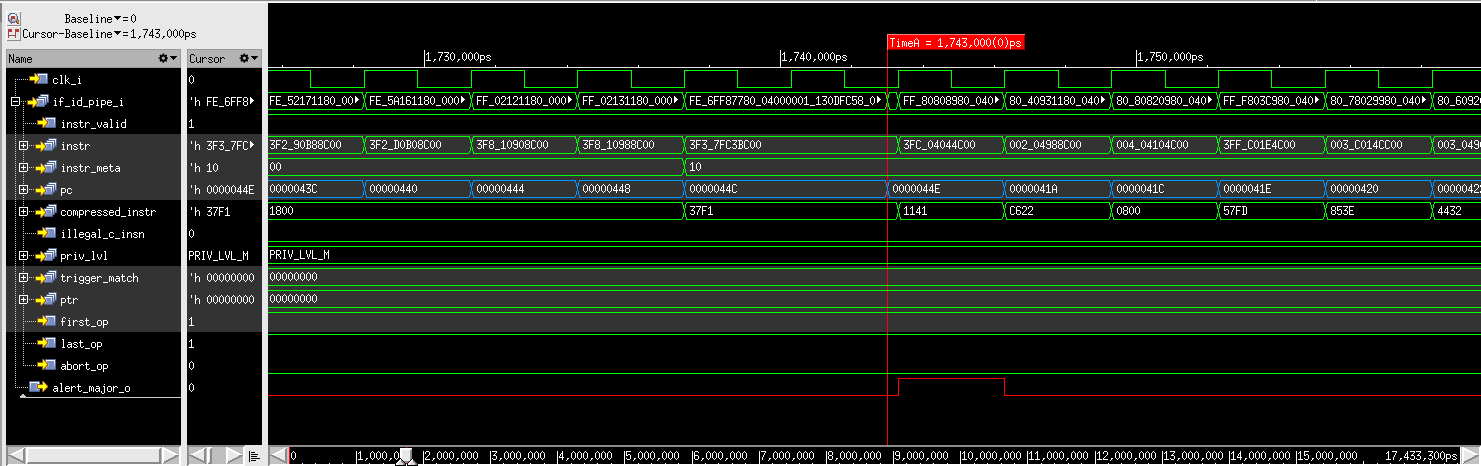
\includegraphics[width=\textwidth]{docs/images/instr_skip_glitch_injection_single_core.png}
    \caption{Waveforms from simulated instruction skip on CV32E40S.}
    \label{fig:instr_skip_single_wave}
\end{figure}

\subsubsection{Skipping out of while loop}

The call to the \textit{c.j} instruction occurs first at 1833ns. The program counter is glitched to be \textit{0x0000047c}.

Glitching out of the while loop was not successful. The attempted instruction skip is detected and a major alert is raised. This can be seen in the simulation waveforms in \autoref{fig:instr_skip_loop_single_wave}. 

\begin{figure}[h!]
    \centering
    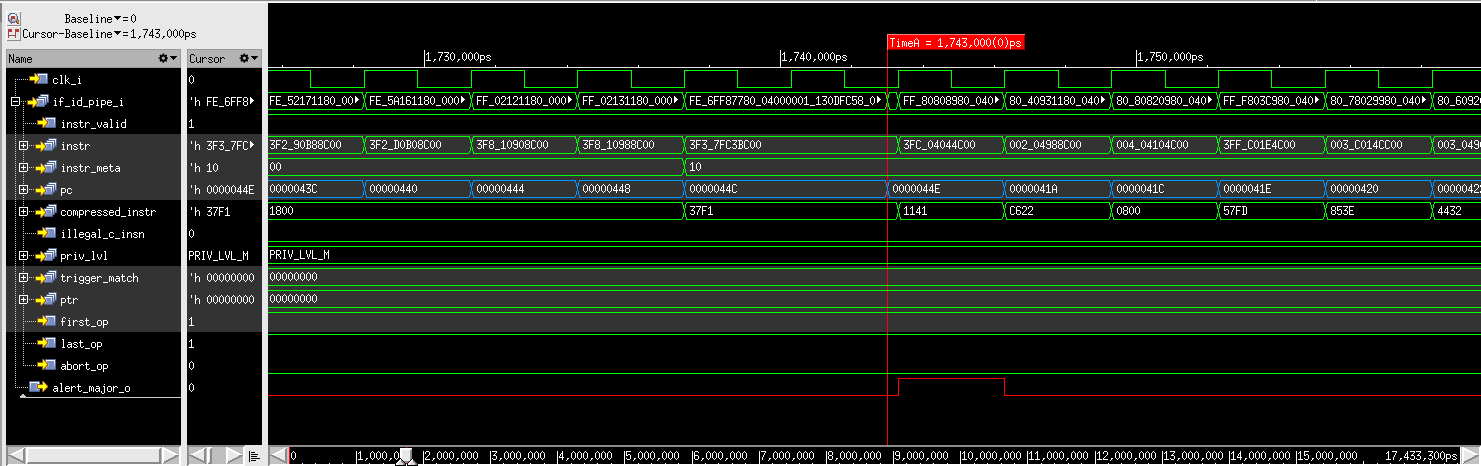
\includegraphics[width=\textwidth]{docs/images/instr_skip_glitch_injection_single_core.png}
    \caption{Waveforms from simulated instruction skip out of loop on CV32E40S.}
    \label{fig:instr_skip_loop_single_wave}
\end{figure}

\subsubsection{Skipping directly to end}

As mentioned earlier, an attacker can potentially glitch directly to the end of the program if they have some way of manipulating the code in the boot-loader. To simulate this, the program counter is forced to the address of the instruction after the while loop, \textit{0x00000482}. This force happens as soon as the main program is entered, which is at 1737ns.

This glitch attack was not successful. However, no major alert was raised by the core as can be seen in \autoref{fig:direct_skip_single_wave}. This glitch therefore bypassed the PCH feature. 

\begin{figure}[h!]
    \centering
    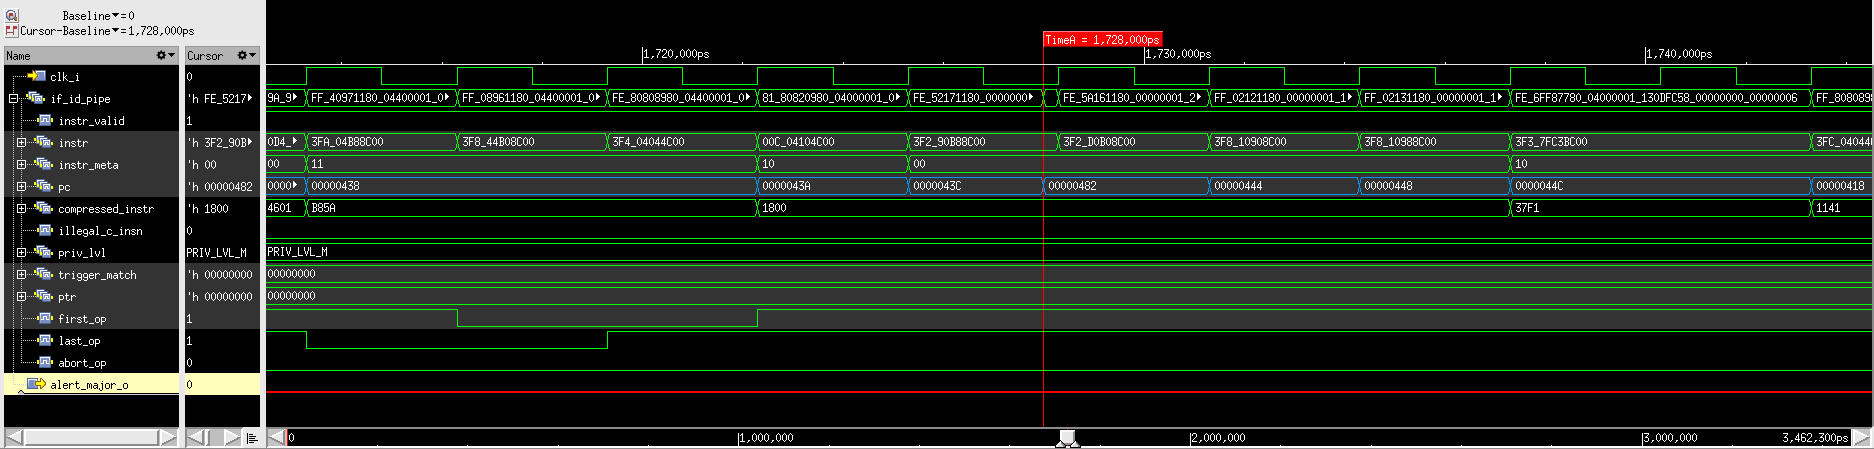
\includegraphics[width=\textwidth]{docs/images/direct_skip_single_core.png}
    \caption{Waveforms from simulated direct instruction skip on CV32E40S.}
    \label{fig:direct_skip_single_wave}
\end{figure}

\subsection{Dual-Core Lockstep}
\label{subsec:dual_instr_skip}

\subsubsection{Skipping function call}

The call to the \textit{c.jal} instruction occurs at 1707ns. The program counter is glitched to the address \textit{0x0000044e}. 

The glitch attack was not successful. From \autoref{fig:instr_skip_loop_dual_wave} we observe that the fault is detected immediately and the error propagates through each stage of the pipeline. 

\begin{figure}[h!]
    \centering
    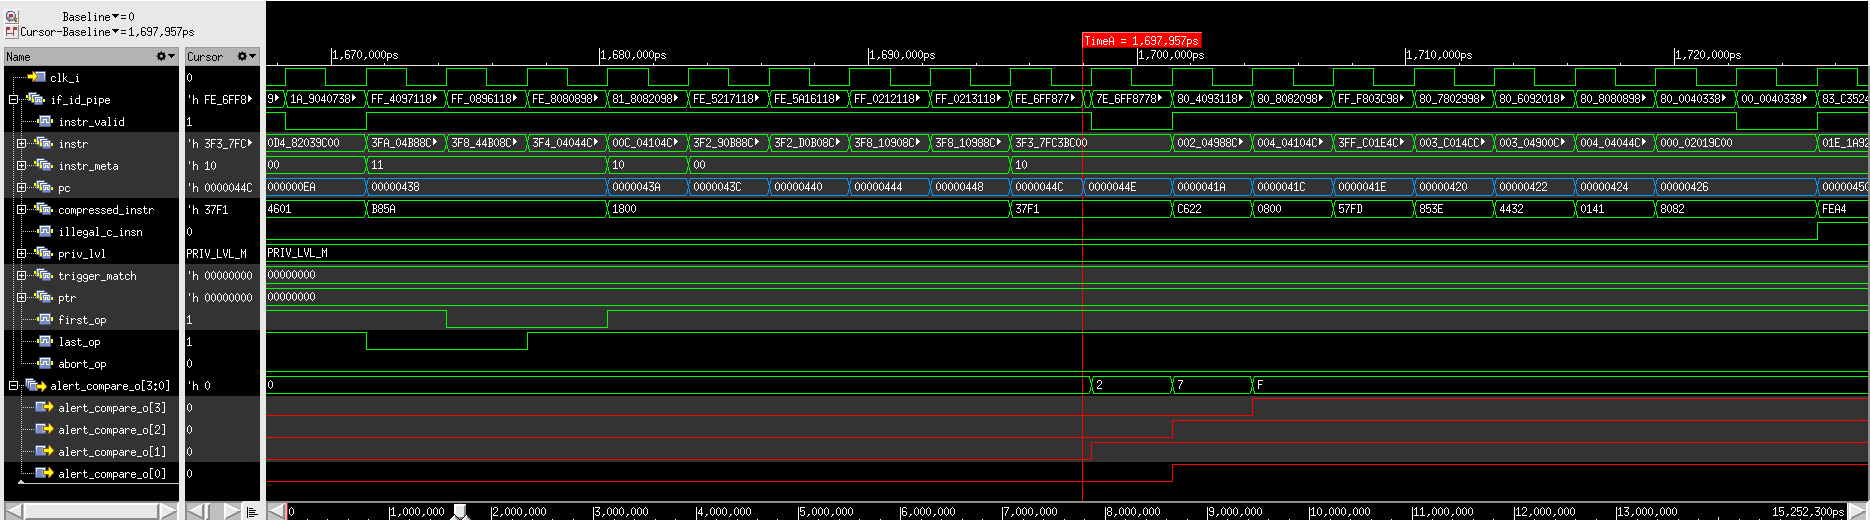
\includegraphics[width=\textwidth]{docs/images/instr_skip_dual_core.png}
    \caption{Waveforms from simulated instruction skip on Dual-Core Lockstep setup.}
    \label{fig:instr_skip_dual_wave}
\end{figure}


\subsubsection{Skipping out of while loop}

The call to the \textit{c.j} instruction occurs first at 1782ns. The program counter is glitched to the address \textit{0x0000047c}.

The glitch attack was not successful. From \autoref{fig:instr_skip_loop_dual_wave} we observe that the fault is detected immediately and the error propagates though each stage of the pipeline. 

\begin{figure}[h!]
    \centering
    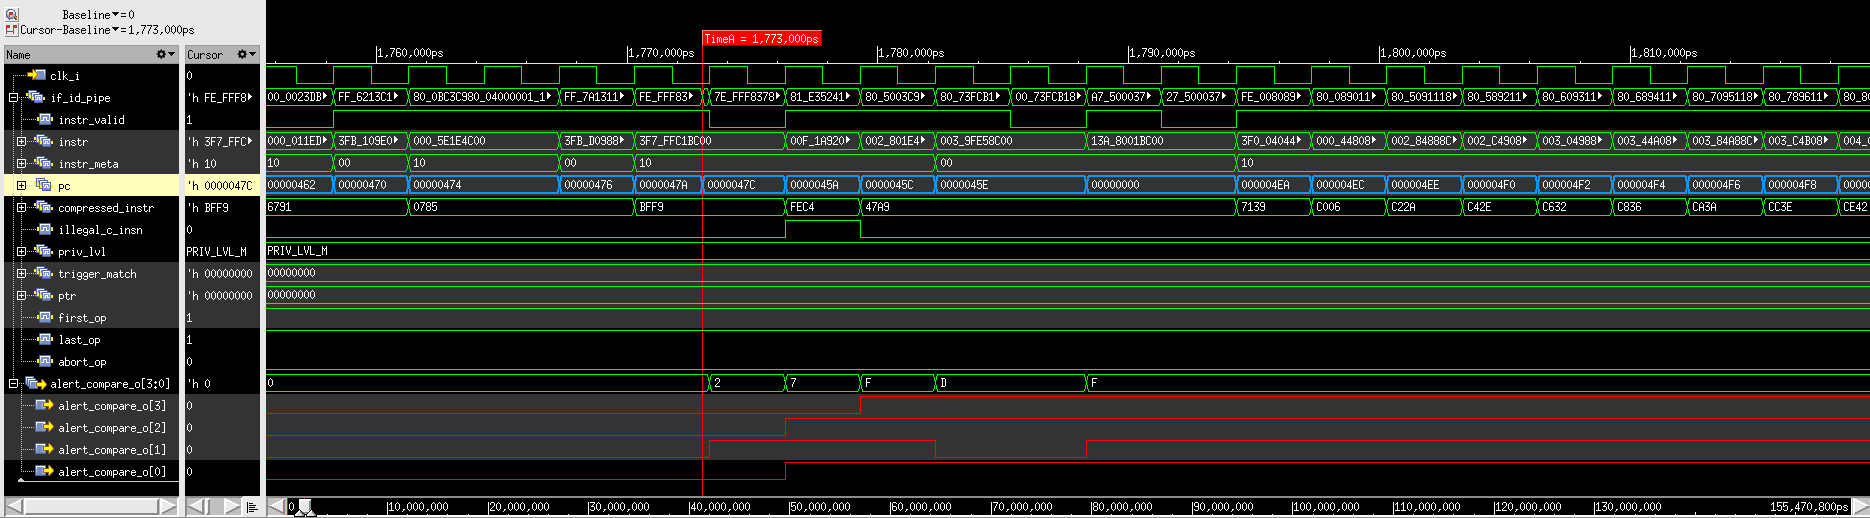
\includegraphics[width=\textwidth]{docs/images/instr_skip_loop_dual_core.png}
    \caption{Waveforms from simulated instruction skip out of loop on Dual-Core Lockstep setup.}
    \label{fig:instr_skip_loop_dual_wave}
\end{figure}

\subsubsection{Skipping directly to end}

The call to the \textit{main} function occurs at 1689ns. The program counter is glitched to the address \textit{0x00000482}.

The glitch attack was not successful. However, unlike in the single core setup a fault is detected and propagated though each stage of the pipeline as can be seen in \autoref{fig:direct_skip_dual_wave}. 

\begin{figure}[h!]
    \centering
    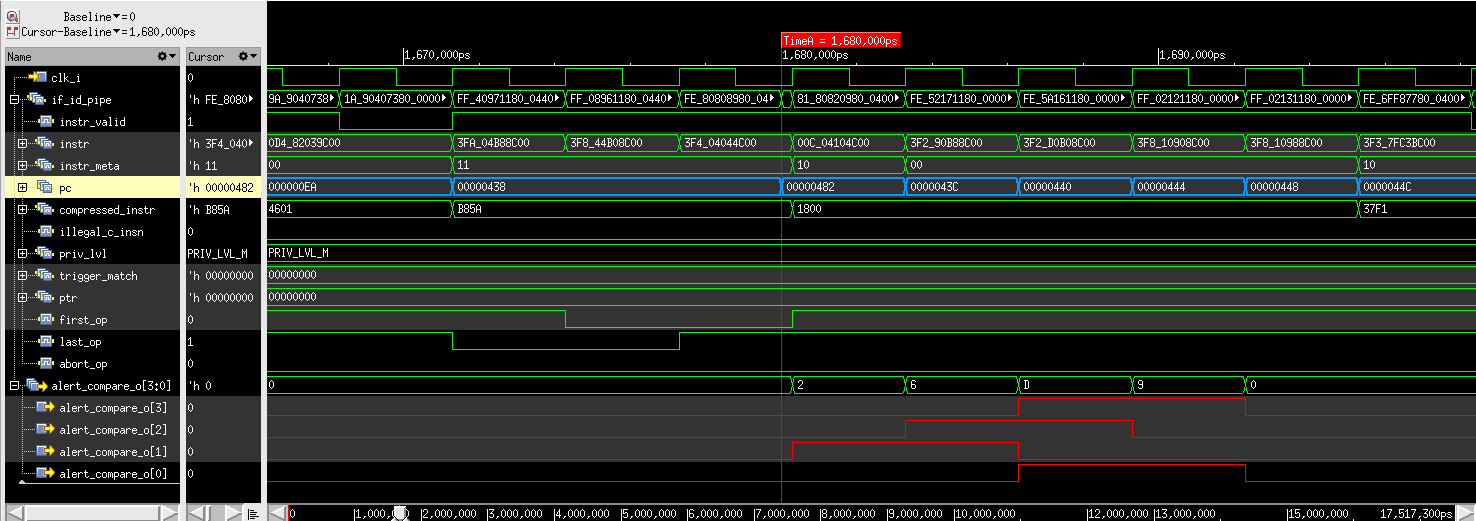
\includegraphics[width=\textwidth]{docs/images/direct_skip_dual_core.png}
    \caption{Waveforms from simulated instruction skip on Dual-Core Lockstep setup.}
    \label{fig:direct_skip_dual_wave}
\end{figure}


\section{Coverage Test}
\label{sec:cov_test_result}

To perform the coverage tests described in \autoref{tab:coverage_test}, the data-bus is glitched in different places in the pipeline. The \textit{store} and \textit{load} instructions are glitched in the \textit{WB} stage as the data is being read or written to the data memory. While three instructions are mentioned in the table, it is only necessary to glitch one of them as the outcome will be similar. Therefore only the instructions corresponding to line \textbf{7} in \autoref{lst:coverage_test} will be glitched. 

\subsection{CV32E40S}

\subsubsection{Glitching load instruction}

This instruction occurs at 1827ns. 

The glitch attack was successful and no major alert was raised by the single core. 

\subsubsection{Glitching store instruction}

This instruction occurs at 1836ns. 

The glitch attack was successful and no major alert was raised by the single core. 


\subsection{Dual-Core Lockstep}

\subsubsection{Glitching load instruction}

\subsubsection{Glitching store instruction}

